% to sort

% os system on mac 
% G4 materials underscores
% wrtten in python 2.7 but in process of being converted to python 3 due to support
% sphere coord needs middlie red line to get slice count consistent
% torus diagram needs colour
% bdsim shooting particles at geant4 sphere and then new old mesh with incresing desities
% then bdsim of compound solids
% mention wether software are free ?
% backwards quotation marks
% equations for motion of a particle
% need to have local copy of code if it changes in appendix listings
% polycone stack kept at 3
% conversion typically leads to leads to loss of detail -> pyg4ometry and GUIMesh are free (open-source) alternatives to this 
% figure to has a y offset , not at centre
% radiation analysis for space craft
% Geometry Description Markup Language (GDML) (G4's format) based on XML.
% The Exchange of Product data (STEP) files
% portugal paper ref
%  Geant4 is a C++ object-oriented toolkit

\documentclass[12pt,a4paper]{article}
\usepackage{graphicx}
\usepackage{hyperref}   
\usepackage{braket}
\usepackage{amsmath}

\usepackage[utf8]{inputenc}
\usepackage[english]{babel}

\usepackage{listings}
\usepackage{color}
\usepackage[margin=0.75in]{geometry}
\usepackage{subfigure}

\definecolor{mygreen}{rgb}{0,0.6,0}
\definecolor{mygray}{rgb}{0.5,0.5,0.5}
\definecolor{mymauve}{rgb}{0.58,0,0.82}
\usepackage{afterpage}

\newcommand{\ts}{\textsuperscript}
\usepackage[super]{nth}
\usepackage{gensymb}
\usepackage{xcolor}
\usepackage{wasysym}
%\usepackage{wasysym} %for astro symbols

 \lstset{ 
  backgroundcolor=\color{white},  % choose the background color; you must add \usepackage{color} or \usepackage{xcolor}; should come as last argument
  basicstyle=\footnotesize,             % the size of the fonts that are used for the code
  breakatwhitespace=false,            % sets if automatic breaks should only happen at whitespace
  breaklines=true,                          % sets automatic line breaking
  captionpos=b,                             % sets the caption-position to bottom
  commentstyle=\color{mygreen},   % comment style
  deletekeywords={...},                   % if you want to delete keywords from the given language
  escapeinside={\%*}{*)},             % if you want to add LaTeX within your code
  extendedchars=true,                    % lets you use non-ASCII characters; for 8-bits encodings only, does not work with UTF-8
  frame=single,	                            % adds a frame around the code
  keepspaces=true,                         % keeps spaces in text, useful for keeping indentation of code (possibly needs columns=flexible)
  keywordstyle=\color{blue},            % keyword style
  language=Octave,                         % the language of the code
  morekeywords={*,...},                  % if you want to add more keywords to the set
  numbers=left,                               % where to put the line-numbers; possible values are (none, left, right)
  numbersep=5pt,                            % how far the line-numbers are from the code
  numberstyle=\tiny\color{mygray},   % the style that is used for the line-numbers
  rulecolor=\color{black},                 % if not set, the frame-color may be changed on line-breaks within not-black text (e.g. comments (green here))
  showspaces=false,                        % show spaces everywhere adding particular underscores; it overrides 'showstringspaces'
  showstringspaces=false,               % underline spaces within strings only
  showtabs=false,                           % show tabs within strings adding particular underscores
  stepnumber=2,                             % the step between two line-numbers. If it's 1, each line will be numbered
  stringstyle=\color{mymauve},        % string literal style
  tabsize=2,	                             % sets default tabsize to 2 spaces
  title=\lstname                               % show the filename of files included with \lstinputlisting; also try caption instead of title
} 

\usepackage{multicol}
\usepackage[font=small,labelfont=bf]{caption} % Makes the font for figure captions smaller and the figure label bold.

\begin{document}
%\pagecolor{black}\afterpage{\nopagecolor}
%\color{white}
\begin{titlepage}
	\centering
	
\includegraphics[width=0.4\textwidth]{Images//Logos//rhul.jpg}\par\vspace{1cm}


	{\scshape\LARGE Royal Holloway University of London \par}
	\vspace{1cm}
	{\scshape\Large PH4100: Major Project\par}
	\vspace{1.5cm}
	{\huge\bfseries Meshing of Primitive Solids\\
	in\\
	Pyg4ometry \& BDSIM\par}
	\vspace{2cm}
	{\Large\itshape Ben Shellswell\par}
	\vfill

\begin{abstract}
\centering

\end{abstract}
The testing and analysis of radiation through the geometries of new concepts and devices, such as a medical magnets, spacecraft or a new particle accelerator, is often a very expensive and time consuming process. The open-source software packages Pyg4ometry \& BDSIM are designed to enable scientists and people within in the industry to virtually simulate these tests, with accurate physics concepts. This project looks at improving the 3D simulation of the events and devices, by remeshing the basic primitive solids.

	\vfill
	
	Supervised by\par
	Prof.~S \textsc{Boogert} 

% Bottom of the page
	{\large \today\par}



\begin{figure}[h]
\centering
\begin{minipage}{.6\textwidth}
  
\includegraphics[width=0.4\textwidth]{Images//Logos//BDSIM_Logo.jpg}
\end{minipage}%
\begin{minipage}{.6\textwidth}
  \centering
  
\includegraphics[width=0.5\textwidth]{Images//Logos//JAI_Logo.jpeg}
  \end{minipage}
\end{figure}

\end{titlepage}
\leavevmode\thispagestyle{empty}\newpage
%\color{black}
\tableofcontents
\thispagestyle{empty}
\newpage
\onecolumn

%%%%%%%%%%%%%%%%%%%%%%%%%%%%%%%%%%%%%%%%%%%%%%%%%%%%%%%%%%%%%%%%%%%%%%
\small
\setcounter{page}{1}

% ------------------------------------------------------------------------------------------------------------------------------

\section{Introduction}

\subsection{Project Aims}
The aims of this project are to contribute towards the optimization of the Pyg4ometry package \ref{pyg} (and subsequently BDSIM \ref{bdsim}), by improving parts of the code and conducting performance test to produce results that can be analysed. The main areas for improvement and where most of the computational energy in wasted, is in the meshing of the primitive Geant4 \ref{g4} compatible solids, due to the unessescary use of boolean operations \ref{bool}.

\subsection{Report Structure}
The subsequent sections are constructed in the following way, the software packages that are used and referenced through out this report (Section \ref{packs}), the concept and details of the primitive meshing used in Pyg4ometry (Section \ref{prim}), then a conclusion and summary of the results of the report (Section \ref{conc}).


% ------------------------------------------------------------------------------------------------------------------------------

\section{Software Packages}
\label{packs}
This section goes through each package of software related to and used throughout the duration of the project. It outlines the key details of each package, describing its function and link to the project. At the time of the project a lot of the prerequisite packages were only compatible with linux systems. Due to owning a windows device, a lot of time was first spent setting up virtual machines running Cent0s 7 (standard free linux used by CERN). However despite getting it setup, the packages were not performing nearly as well as they were on the macs, therefore for the duration of project a loaner linux laptop (2011 Apple MacBookPro running OS El Capitan) was used from the particle physics department of Royal Holloway. 

\subsection{BDSIM}
\label{bdsim}
BDSIM (or Beam Delivery SIMulation) is a open source software package written by the John Adams Institute (JAI) \cite{jai}, for the use of modelling particle beam interactions. BDSIM has many applications, such as modelling complex particle accelerators for example the Large Hadron Collider (LHC) or concepts magnets for medical scanners used to treat tumors. The package allows a user to specify the physics being used for a particular particle of a set energy colliding with a provided object. The scattering of the particle trajectories and decays are computed using Monte Carlo simulations, to make the results as consistent with experimental results as possible. The software outputs a full analysis of each run, and can even allow multiple runs to run at once (batch mode).

\subsection{Pyg4ometry}
\label{pyg}
Pyg4ometry is an open source python package also generated by JAI, its purpose is to convert 3D CAD (Computer Aided Design) models between different representations to allow compatibility with BDSIM for the testing of new concepts. The '4' in 'Pyg4ometry' comes from the consistency the package has with Geant4 \ref{geant4}. The package is a key tool for allowing multiple file formats to become compatible with BDSIM, which increases the number of people who can utilise the package.
\\\\
Most of the development in this project is conducted in Pyg4ometry and managed using an online git in combination with Sourctree. The package is currently written in and only supports Python 2.7, however as of January 2020 Python 2 is no longer being backed as a the newer version Python 3 is taking over. The transition to Python 3 means adjusting the syntax of several functions and files in Pyg4ometry, this has began but a full transition will take sometime as it is not an immediate priority.

\subsection{Geant4}\label{geant4}
\label{g4}
Geant4 (or GEometry ANd Tracking) is a software developed in C++ for the simulation and tracking of particles traveling through matter. The package is used by many particle physicists and is one of the more popular options for handling the geometry within interactions. Geant4 has its own preset solids that are used for simulating particle interactions. For ease of conversion between file formats Pyg4ometry uses the same conventions when meshing its primitive solids.
\\\\
The materials used in Pyg4ometry and throughout this project are also from the Geant4 database. In this report the three main materials used are $G4_Fe$, $G4_Ti$ and $G4_Galactic$ (Iron,Titanium and Vacuum). The use of $G4_Galactic$ is the most important as it is used to set the material of the world environment in with other objects are placed into. By default the World material in BDSIM is set to be air, which meant the particles would interact with the air before passing into the object being tested, this was avoided by using the option $worldMaterial="G4_Galactic"$ withtin the $.GMAD$ files.

\subsection{ROOT}\label{root}
Root files are the default output for analysis by BDSIM, as it has been heavily used by particle physicists since its release. Root has its own file browsing system due to the nature of its formatting. Root is adopted by many physics communities such as CERN \cite{cern}, where it was first written.

\subsection{Freecad (Libraries)}
FreeCAD 0.18 \ref{}.

\subsection{Visulisation Packages}
VTK\\
Geant4\\
BDSIM\\
FreeCAD\\

% ------------------------------------------------------------------------------------------------------------------------------
\newpage
\section{Primitive Meshing}
\label{prim}
This section will describe the work done to optimize the python scripts that generate the three dimensional meshing for the primitive solids within the Pyg4ometry package \ref{pyg}. All the primitive solids used are constructed such that they are compatible with Geant4's solids. It was orginally thought that it would be best to use triangular based meshes in combination with boolean operations \ref{bool} to construct the 3D solids. However it has been realised that the computation of triangles and boolean operations compared with polygons and adapted trigonometry is much more intensive and inefficient, in most cases. In particular with the curved solids, i.e circular and elliptical based solids.
\\\\
One of the major improvements to the Pyg4ometry \ref{pyg} code is the computation of cut up primitive solids. The meshing of hollow or sliced solids were previously computed by Boolean subtractions and unions, which involved creating two separate solids and acting upon both of them. Discussed more in Section \ref{bool}. Which resulted in a very computationally heavy and less aesthetic outcome, where the mesh lines ('slice and stack'), were not meshed in radial directions.

\subsection{Co-ordinate Systems}
The various primitive solids are all constructed by using the predefined parameters used by Geant4 \ref{g4}, to be consistent with Geant4's own solids. The parameters of a 3D solid are properties relating to the coordinate system it is constructed in, such as height or radius. The parameters are then used to define the points of the object via basic trigonometry.
\\\\
The python meshing scripts for all coordinate systems follow a similar structure, of first defining an empty list of faces (polygons). Then running the associated trigonometric equations through a number of loops to generate and append polygons to that list. The number of loops is associated with the number of sections a surface of a solid is being split up into in a given coordinate system. The density of the meshing is defined by a user inputted number of slices and stacks, demonstrated in Figure \ref{cylmeshin}.

\subsubsection{Cylindrical Co-ordinate System}
\label{cycl}
The meshing for the primitive solids in cylindrical polar coordinate systems are constructed by looping though the user defined number of slices and stacks (as shown in Figure \ref{cylmeshin}) which the cylinder is being cut into (Listing \ref{code1}). The Loop then creates the coordinates for 3 or 4 points at a time using an adaption to the trigonometry in Equations \ref{cyctrig}, which can then be defined as a triangular or polygonal face. The only cases where the mesh produces triangles is at the top and bottom faces of the cylinder, provided it does has a minimum radius equal to zero (creating a tube or cone). The same logic for the polygons also applied to triangles, just using 3 vertex points to make a face.

\begin{figure}[h!]
\centering
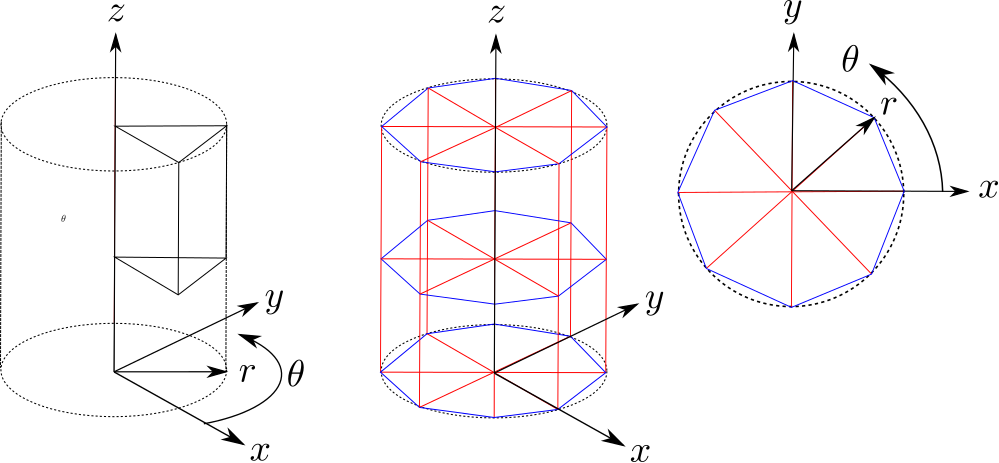
\includegraphics[scale=0.45]{Images//Coords//cyl.png}
\caption[width=\columnwidth]{Diagram showing the meshing method for a cylindrical coordinate system\\
Red = Slices   (8)\\
Blue = Stacks (2)}
\label{cylmeshin}
\end{figure}
\vspace{0.3cm}
The trigonometry that converts the points from cylindrical polar coordinates to cartesian, are:
\begin{equation}
\begin{aligned}
\label{cyctrig}
& x = r \cos{\theta} \\
& y = r \sin{\theta} \\
& z = z
\end{aligned}
\end{equation}

%\label{code1} 
\newpage
\begin{lstlisting}[language=Python, label=code1, caption=Basic method structure for Pyg4ometry primitive meshing of solids]
polygons = []

for j0 in range(nslice):
    j1 = j0
    j2 = j0 + 1
    
    vertices = []

    for i0 in range(nstack):
          i1 = i0
          i2 = i0 + 1     

\end{lstlisting}
The code in Listing \ref{code1} generates counters so that you can choses from two slices and two stacks, in order to gain the four points surrounding a desired face. These points are then used to define a polygon. 
\\\\
The only time a stack is needed in the cylindrical coordinate system is when the solid has a non linear function in the r-z plane. For example a paraboloid (Figure \ref{para}) would need a stack, but a linear cone (Figure \ref{cons}) would not. This is due to the fact how that a plane can't represent a curved surface with a singe face. 

\newpage
\subsubsection{Spherical Coordinate System}

The meshing for the primitive solids in spherical coordinate systems are constructed by similar means the that of the cylindrical \ref{cycl}. Just with different trigonometric equations (Equations \ref{trigsph}) as a result of two angle parameters $\phi$ and $\theta$. The stack (blue) and slice (red) for solids in the spherical coordinate system works, like the longitude and latitude on a globe, as shown in Figure \ref{sphmeshin}. 
\\\\
The trigonometry that converts the points from spherical coordinates to cartesian, are:

\begin{equation}
\begin{aligned}
& x = r \cos{\theta}\sin{\phi}\\
& y = r \sin{\theta}\sin{\phi} \\
& z = z
\end{aligned}
\label{trigsph}
\end{equation}
\begin{figure}[h!]
\centering
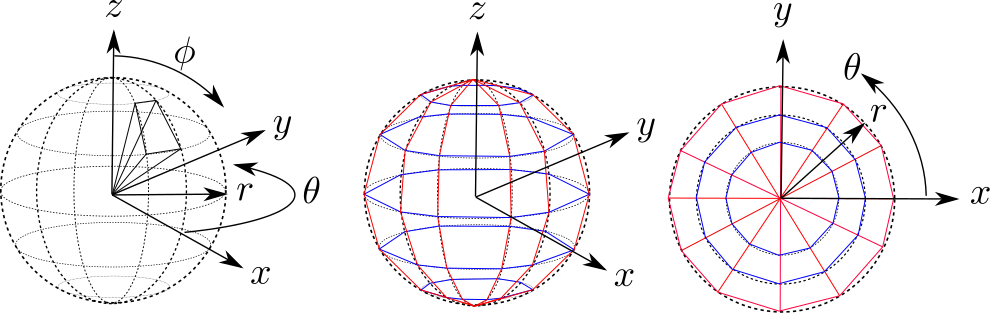
\includegraphics[scale=0.5]{Images//Coords//sph.png}
\caption[width=\columnwidth]{Diagram showing the meshing method for a spherical coordinate system\\
Red = Slices (12)\\
Blue = Stacks (6)}
\label{sphmeshin}
\end{figure}

\noindent The structure of the code is the same as used in Listing \ref{code1}.\\\\
\noindent The only time triangles are constructed in the spherical coordinate system is if the solid has a complete pole at the top or bottom of the solid. The solids constructed in the spherical always have both a stack and a slice.

%\begin{lstlisting}[language=Python, caption=Python example]
%for j0 in range(nslice):
%    j1 = j0
%    j2 = j0 + 1
%
%    for i0 in range(nstack):
%          i1 = i0
%          i2 = i0 + 1
%\end{lstlisting}

\newpage
\subsubsection{Toroidal Coordinate System}

A toroidal shape is much harder to visualise a stack and slice, due to the fact it is a rotating coordinate system. A toroidal slice is an $R_{Torus}$ radial cut taken out of the angle $\phi$, as shown in Figure \ref{tormeshin}. The toroidal stack is a $R$ radial cut out of the angle $\theta$. 
\\\\
The trigonometry that converts the points from toroidal coordinates to cartesian, are:

\begin{equation}
\begin{aligned}
& x = R_{Torus} + R\cos{\theta}\cos{\phi} \\
& y = R_{Torus} + R\cos{\theta}\sin{\phi} \\
& z =  R\sin{\theta} 
\end{aligned}
\end{equation}

\begin{figure}[h!]
\centering
\includegraphics[scale=0.35]{Images//Coords/torus_coords.png}
\caption[width=\columnwidth]{Diagram showing the meshing method for a toroidal coordinate system}
\label{tormeshin}
\end{figure}

\subsection{Plane Direction}
One key thing to be taken into account is the convention being used in the code for the order in which points are appended to make a plane, i.e to define a face on a solid. This is important as the direction the normal of the plane points in, dictates wether a face is considered an inside or outside face on the given solid. Getting this incorrect, will lead to missing faces, when the meshing is made. The concept is demonstrated in Figure \ref{pointsorder}.

\begin{figure}[h!]
\centering
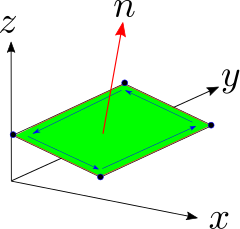
\includegraphics[scale=0.75]{Images//append_points//Point_Appending_Order.png}
\caption[width=\columnwidth]{Diagram showing the order convention of appending points to define the normal to a plane}
\label{pointsorder}
\end{figure}
\noindent The simplest way to test this is by performing boolean operations with a box, as the boolean operation will only work nicely if all the planes are correct on both shapes.

\subsection{New Meshing of Curved Primitive Solids}
In total there are 12 curved primitive solids, of which many of the examples and concepts are very similar. Therefore only a few solids will be discussed in this section, but their development can all be viewed in Appendix \ref{app1}.
\\\\
can give one example and reference rest in appendix, radial meshing clean up, can remove stack in some cases, boolean slow and messy

\begin{figure}[h!]
\centering
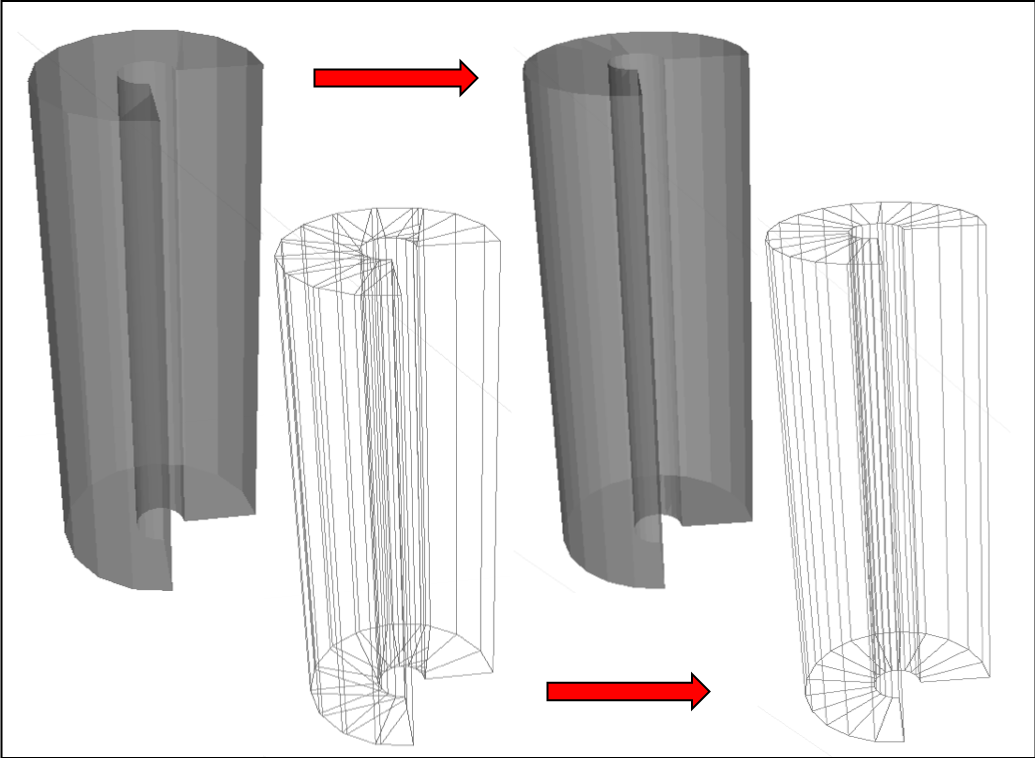
\includegraphics[scale=0.5]{Images//Meshes//tubs.png}
\caption[width=\columnwidth]{Meshing Development for Tubs (Solid \& Mesh View)}
\label{tubspic}
\end{figure}

\subsubsection{Degenerate Points}
Multiple meshing points occupying the same area can spring a few errors, sometimes without entirely crashing the code, making it a hard error to identify. I is typically given away when a $DivisionByZero$ error occours, within the pycsg meshing of a solid. You can identify wether this is the error by debugging each polygon and triangle in a mesh, looking out for a face that has two or more vertices with the same $(x,y,z)$ coordinates.

\subsubsection{Boolean Operations}
\label{bool}
One of the largest improvements to the performance of the new meshing methods compared with the previous methods, is the discarding of boolean operations in order to create hollow or cut-up primitive solids. The idea can be clearly seen in Figure \ref{booly}, where you conduct basic operations on simple solids, resulting in a complex solid being made.
\\
\begin{figure}[h!]
\centering
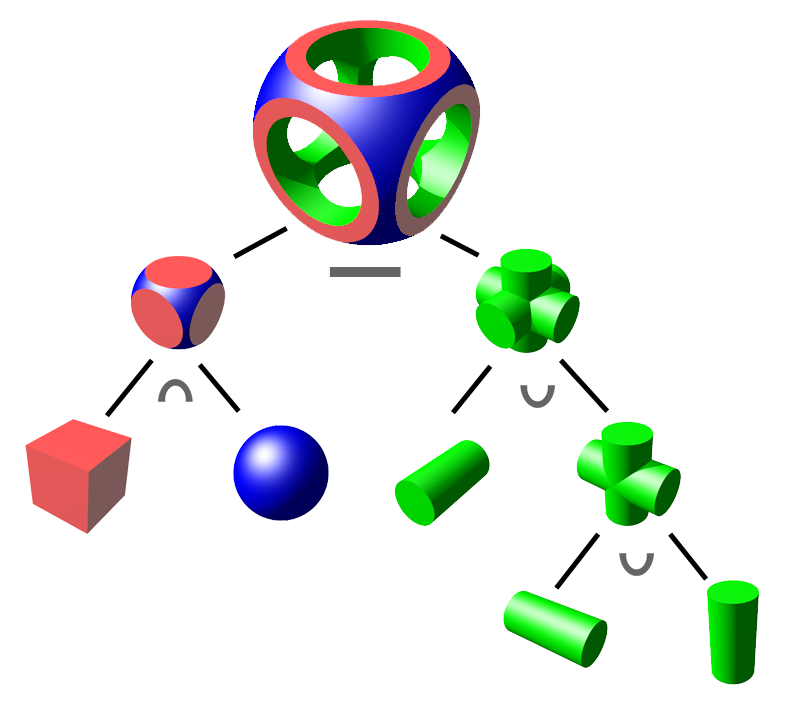
\includegraphics[scale=0.3]{Images//Booleans//Boolean.png}
\caption[width=\columnwidth]{A diagram showing the basic method of constructing a more complicated 3D solid out of boolean operations with simpler primitive solids.}
\label{booly}
\end{figure}

\noindent The Figures \ref{uni} \& \ref{sub} are of the meshed boolean union and subtraction of a box with a hollow sphere (in solid view). The coloured lines are representing the perpendicular planes in which the final object is place in. These were made in the process of checking the normals before passing them into BDSIM.
\\
\begin{figure}[h!]
\centering
\begin{minipage}{.4\textwidth}
  \centering
  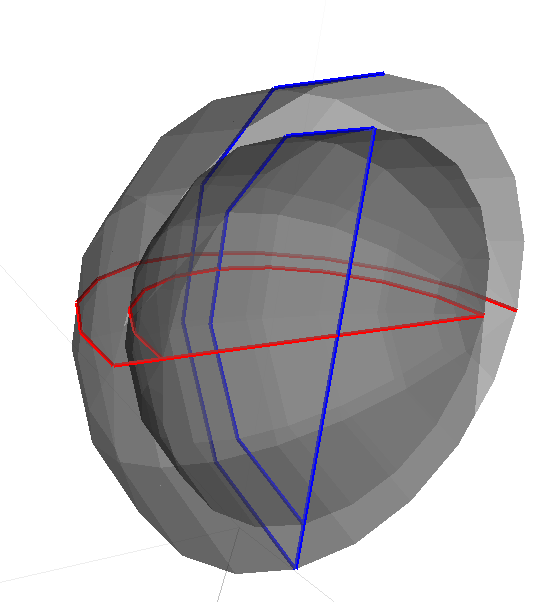
\includegraphics[height=0.5\linewidth]{Images//Booleans/SphereUnion.png}
  \captionof{figure}{Example screenshot of\\ a Boolean Union produced in\\ Pyg4ometry.}
  \label{uni}
\end{minipage}%
\begin{minipage}{.4\textwidth}
  \centering
  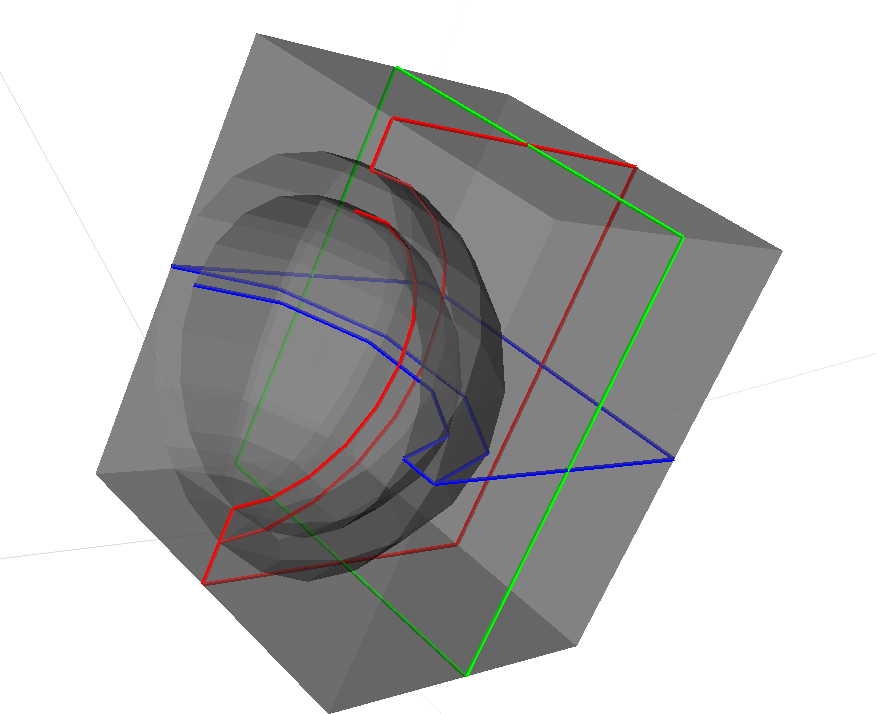
\includegraphics[height=0.5\linewidth]{Images//Booleans//SphereSubtraction.png}
  \captionof{figure}{Example screenshot of \\ a Boolean Subtraction produced\\ in Pyg4ometry.}
  \label{sub}
\end{minipage}%
\end{figure}



\noindent The old meshing algorithms would heavily rely on these operations. The old meshing algorithms used intersections to slice solids Figure \ref{ctub} and subtractions to make solids hollow of cut-up Figure \ref{Sphere}. For example Tubs is made from two cylinders being subtracted in order to create a tube as seen in Figure \ref{tubspic}. The boolean operations worked, however are very computationally heavy compared with that of the adapted trigonometry applied in the new method. Another thing the boolean operations affected was the appearance of the mesh its self, the boolean operations worked by trying to identify common mesh points and then remeshing. This created a lot of non radially uniform mesh sections as seen in Tubs.\\



\newpage
\subsection{Meshing Performance Testing}
\subsubsection{Polygon Count}
One way in which the meshing performance of the Pyg4ometry primitive solids is conducted, is by counting the number of polygons produced by both the old and new meshings, in order to make a comparison. A plot for each primitive solid counting its number of generated polygons was produced. They were generated by varying the user inputted number of slices across a range. Most were put through the range of (10-100) slice whilst keeping the number of stacks at a constant 10. However a few old solid meshings took so long to produce at higher mesh densities, they were only measured across shorter ranges e.g the old Hyperboloid meshing was left to run for over an hour.  \\

\begin{figure}[h!]
\centering
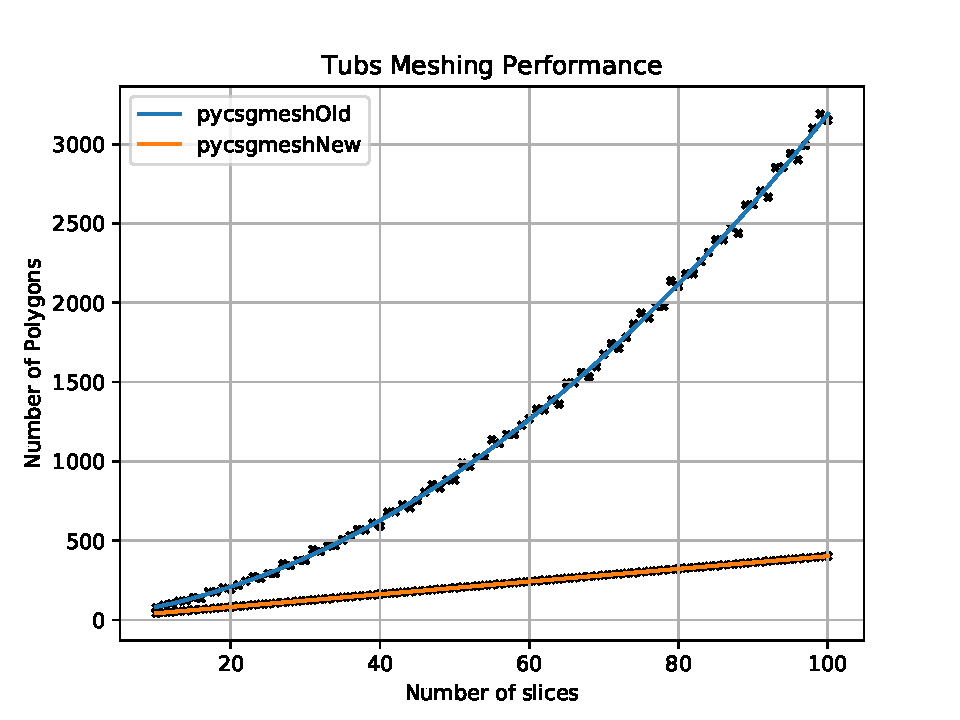
\includegraphics[scale=0.6]{Images//Quad_fits//Tubs_quad.pdf}
\caption[width=\columnwidth]{A plot showing the comparison of the number of polygons (and triangles) generated by the new and old meshing methods, across a range of slices 10-100.}
\label{conts}
\end{figure}

\noindent The polygon count plots for the remaining primitive solids can be found in the Appendix \ref{app1}. A table of parameters for the quadratic fits can also be found in the Appendix \ref{tab1}. 

\newpage
\section{BDSIM Interactions}
The second aim of this project was to measure how the physics is altered, between the new and old meshings as the mesh density is varied. Geant4 already has its own set of primitive solids, which can be used as a guideline for comparison. The physics being measured will be features such as the trajectories and energy deposition, through solids.
\\\\
Within BDSIM the charge of a particle is represented by its colour, green = neutral, blue = positive and red = negative. The probability of certain events and the scattering of a particles trajectories is generated by a Monte Carlo simulation. Each seed that produces a different outcome in the Monte Carlo simulations has a unique seed number. This allows a particular event to be repeated with the same physics, which is key to this project when it comes to comparing the interactions of two different objects under the same conditions. Other properties of the particle and physics processes that it may undergo can also be user defined to tweak the experiment. Properties such as the particles initial energy, wether secondaries get produced and much more.
\\\\
Each BDSIM event outputs $.root$ file which contains a detailed analysis of the interaction. One of the elements analysed within this project is the energy loss across the Z-axis.
\\\\
BDSIM works by running a $.GMAD$ file and then outputs $.root$ file with the option of a 3D visualisation of the interactions. The $.GMAD$ contains the basic information needed to produce an output, i.e a particle and a target file (Typically of the format $.GDML$).
\\\\
Due to Geant4 already having its own primitive solids, you cannot directly pass a meshed primitive solid into BDSIM without it being replaced with a Geant4 one. The way around this is to pass the mesh into another Geant4 tessellated solid, which intakes the properties of a meshed solid without overriding them with a Geant4 alternative. This proved to be more difficult than first intended due to many of the solids having a mixture of quadrangular and triangular faces to be unpacked. It orginaly sprung a few problems such as missing faces or faces of the wrong shape. 
\\\\
One of the first shapes to be tested in BDSIM was the sphere, which is made of a minimum and maximum radius, making it a hollow solid. As seen in Figure \ref{sphbd} the sphere was chosen to be orientented such that the particle beam is fire from the centre of the sphere outwards. The conversion from a Pyg4ometry mesh into a GDML tessellated solid, results in only triangular faces. This is why all the quadrilateral faces are cut into two in Figure \ref{sphbd}.

\begin{figure}[h!]
\centering
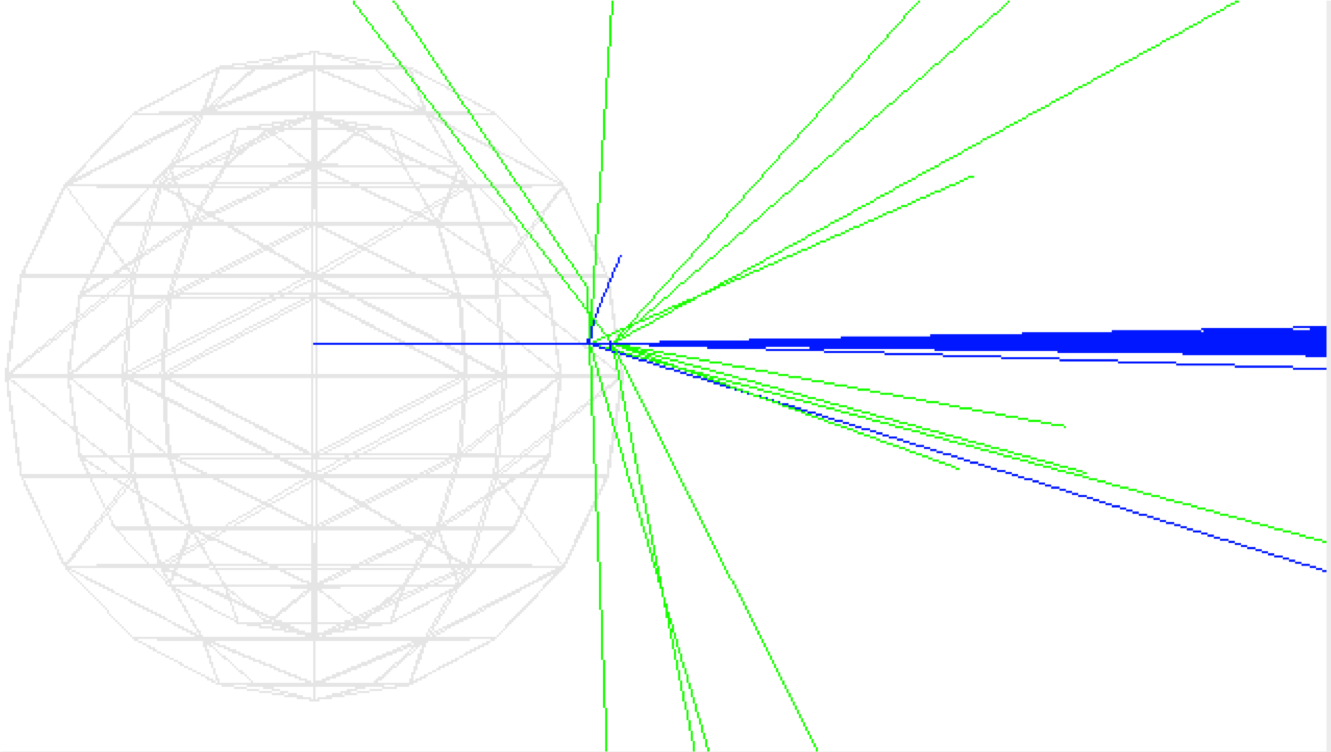
\includegraphics[scale=1]{Images//BDSIM//ProtonSphere.png}
\caption[width=\columnwidth]{BDSIM screenshot of 200 1.3 Gev protons interacting with a Iron sphere, generated with the new meshing using a stack \& slice of 10 \& 10. (Shown in mesh view)}
\label{sphbd}
\end{figure}

\noindent One way that was though to analyse the energy deposition of the interactions, was to look at the CPU duration times as the mesh densities are increased. In this scenario the Geant4 solid was used as a guideline as it does not depend on a user defined stack \& slice. 

\subsection{Iron Sphere Interactions}
rmin = 8mm\\
rmax = 10mm\\
1.3Gev protons\\
10,000\\

\begin{figure}[h!]
\centering
\begin{minipage}{.5\textwidth}
  \centering
  \includegraphics[height=0.75\linewidth]{Images//CPU//Total_plot.pdf}
  \captionof{figure}{A plot showing mean\\ CPU duration of 10,000 protons\\ interacting with a Iron sphere of\\ various meshed forms.\\}
  \label{cons}
\end{minipage}%
\begin{minipage}{.5\textwidth}
  \centering
  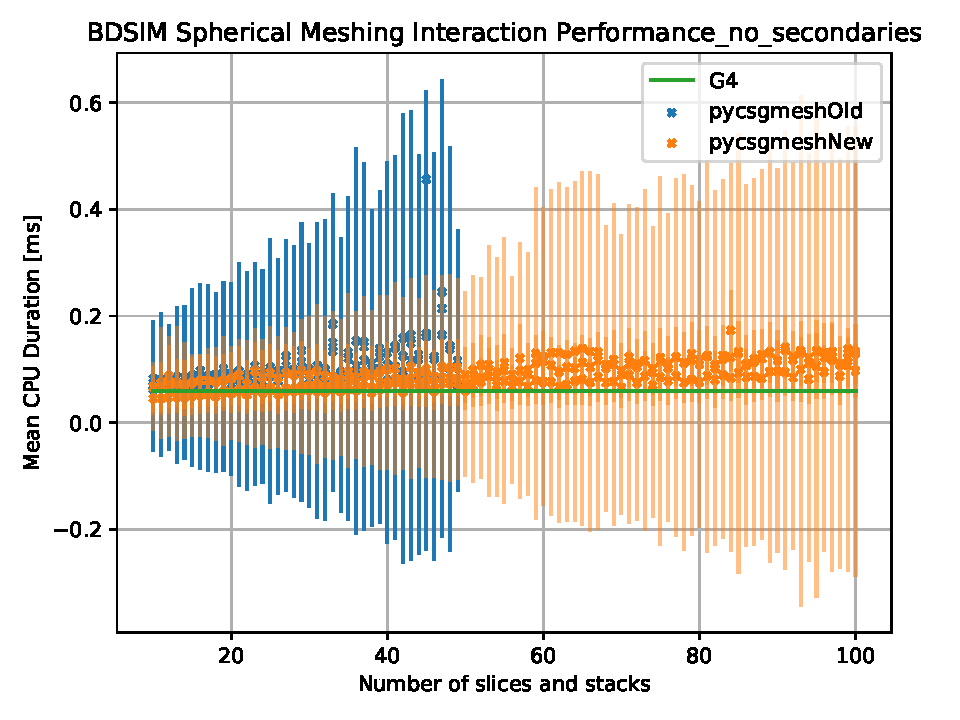
\includegraphics[height=0.75\linewidth]{Images//CPU//Total_Plot_no_secondaries.pdf}
  \captionof{figure}{ A plot showing mean\\ CPU duration of 10,000 protons\\ interacting with a Iron sphere of\\ various meshed forms, with\\ secondary particles disabled.}
  \label{fig:test2}
\end{minipage}%
\end{figure}

\begin{figure}[h!]
\centering
\begin{minipage}{.5\textwidth}
  \centering
  \includegraphics[height=0.75\linewidth]{Images//CPU//Total_plot_with_offset.pdf}
  \captionof{figure}{A plot showing mean\\ CPU duration of 10,000 protons\\ interacting with a Iron sphere of\\ various meshed forms, with\\ an 20mm of set in the Z-axis.}
  \label{cons}
\end{minipage}%
\begin{minipage}{.5\textwidth}
  \centering
  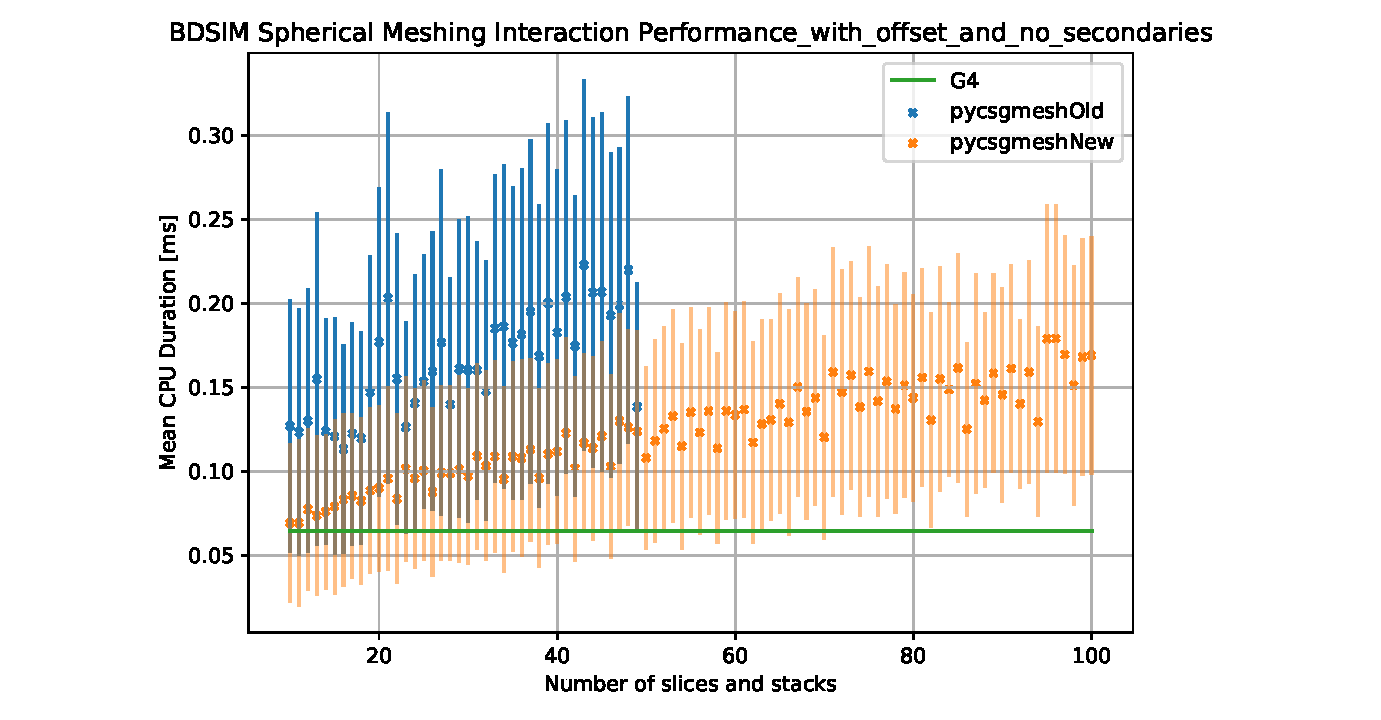
\includegraphics[height=0.75\linewidth]{Images//CPU//Total_Plot_with_offset_and_no_secondaries.pdf}
  \captionof{figure}{ A plot showing mean\\ CPU duration of 10,000 protons\\ interacting with a Iron sphere of\\ various meshed forms, with\\ secondary particles disabled, with\\ an 20mm of set in the Z-axis and secondaries disabled.}
  \label{fig:test2}
\end{minipage}%
\end{figure}

\noindent It was orginaly thought that the standard deviations of the CPU durations was related to the number of secondaries being produced. However this was disproved by Figure \ref{}, where the same test was conducted with the BDSIM option that disables secondary particles from being produced implemented.

\subsubsection{Error Reduction}
To reduce the standard deviation of a data set the number of events needs to be increased, this proved by the relation ship sown in Equations \ref{std}. The relationship between the standard deviation and number of events is inversely square root proportional.

\begin{equation}
\begin{aligned}
& \bar{x} = \frac{1}{N}\sum{x_i}\\
& \sigma = \sqrt{\bar{x}^2} = \sqrt{\frac{1}{N}\sum{(x_i - \bar{x}})^2}\\
& \sigma \propto \frac{1}{\sqrt{N}} 
\end{aligned}
\label{std}
\end{equation}


\subsection{Titanium Sphere Interactions \& Spherical Beam Distribution}
rmin = 0.01mm\\
rmax = 10mm\\
beam dist = sphere\\
10 GeV electrons\\
N decided by reduction\\

\begin{figure}[h!]
\centering
\includegraphics[scale=0.3]{Images//BDSIM//titanium.pdf}
\caption[width=\columnwidth]{Meshing Development for Tubs (Solid \& Mesh View)}
\label{tubspic}
\end{figure}

\subsection{Interaction with Magnet}
As a final goal to round off the project a compund boolean meshed solid of a real world magnet is analysed in the same way in which the meshed sphere was in the previous section. 
\newpage
\section{Conclusion \& Summary}
\label{conc}

\subsection{Improvements}
meshing is quicker\\
BDSIM interactions are quicker but still slower than G4 solid (as expected)
improved coverage unit test speeds\\
meshing is neater and more uniform in structure\\
higher meshing density = closer to true solid as expected with bdsim interactions\\

\subsection{Applications}
BDSIM and Pyg4ometry are both very powerful software packages that can be used to to aid not only the scientific research community of particle physicist, but also help everyday people treat patients. Thanks to the software being open source and its wide range of file compatibilities it can be used to simulate a growing number of projects.

% ------------------------------------------------------------------------------------------------------------------------------


\newpage
\begin{thebibliography}{1}

	\bibitem{}
		BDSIM Manual\\
		\url{http://www.pp.rhul.ac.uk/bdsim/manual/}
	\bibitem{}
		BDSIM Paper\\
		\url{https://doi.org/10.1016/j.cpc.2020.107200}
		
	\bibitem{}
		Pg4ometry BitBucket\\
		\url{https://bitbucket.org/jairhul/Pyg4ometry/src/}
		
	\bibitem{}
	Geant4 Solids\\
	\url{http://geant4-userdoc.web.cern.ch/geant4-userdoc/UsersGuides/ForApplicationDeveloper/html/Detector/Geometry/geomSolids.html}
	
	\bibitem{}
	Geant4 Materials\\
	\url{http://geant4-userdoc.web.cern.ch/geant4-userdoc/UsersGuides/ForApplicationDeveloper/html/Appendix/materialNames.html}
	
	\bibitem{jai}
	JAI\\
	\url{https://www.adams-institute.ac.uk/}
	
	\bibitem{cern}
	CERN\\
	\url{https://home.cern/}
	
	\bibitem{meh}
	M. Pinto, P. Gon\c{c}alves\\
	GUIMesh: A tool to import STEP geometries into Geant4 via GDML\\
	\url{https://doi.org/10.1016/j.cpc.2019.01.024}
		
\end{thebibliography}


% ------------------------------------------------------------------------------------------------------------------------------

\newpage
\appendix

\section{Appendix (Python scripts)}
\subsection{Sphere BDSIM Vary Mesh Test}\label{ap1}
\lstinputlisting[language=Python]{Scripts//Run_New_Meshes.py}

%\newpage
%\subsection{Discovery method contribution pie chart (Figure \ref{pie})}\label{ap2}
%\lstinputlisting[language=Python]{Python//pi.py}

\newpage
\twocolumn[\section{All Meshed Solids and Polygon Count Plots}
\label{app1}
The following Figures are the meshing and polygon data for each primitive solid constructed in Pyg4ometry \ref{pyg}. The first Figure for each solid is screenshots of the old meshing and new meshing visualized in VTK. They show the before and after of each primitive solid in both "solid view" and "mesh view". The second Figures Show the number of polygons and triangles produced by the solid as you increase the slice across a range of 10-100 (if there is a stack it is kept at a constant 10). The polygon data plots are generate using python 2.7. The naming convention is the one used by Geant4 \ref{g4}.\\]
\begingroup
\subsubsection{Cons}
\begin{figure}[h!]
\centering
\begin{minipage}{.2\textwidth}
  \centering
  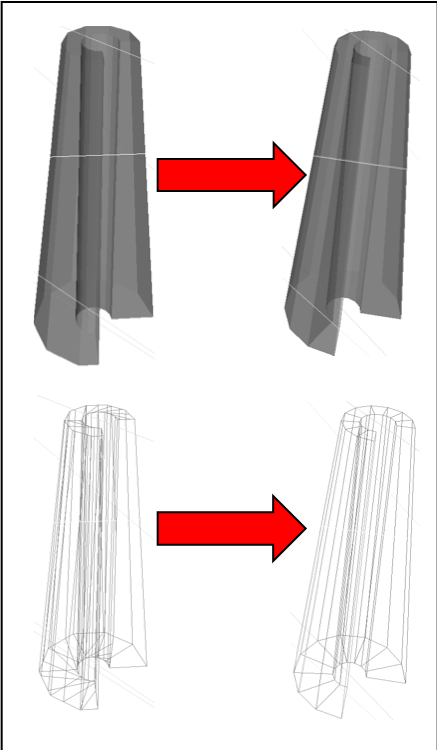
\includegraphics[height=1\linewidth]{Images//Meshes//cons.png}
  \captionof{figure}{}
  \label{cons}
\end{minipage}%
\begin{minipage}{.3\textwidth}
  \centering
  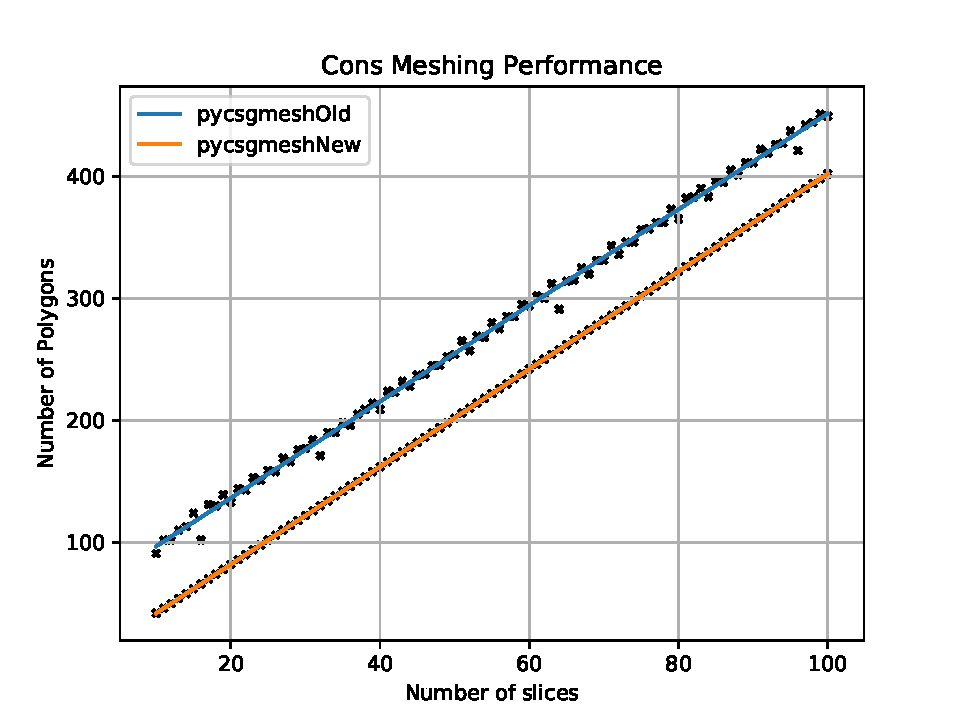
\includegraphics[scale=0.35]{Images//Quad_fits//Cons_quad.pdf}
  \captionof{figure}{ }
  \label{fig:test2}
\end{minipage}%
\end{figure}

\subsubsection{CutTubs}

\begin{figure}[h!]
\centering
\begin{minipage}{.2\textwidth}
  \centering
  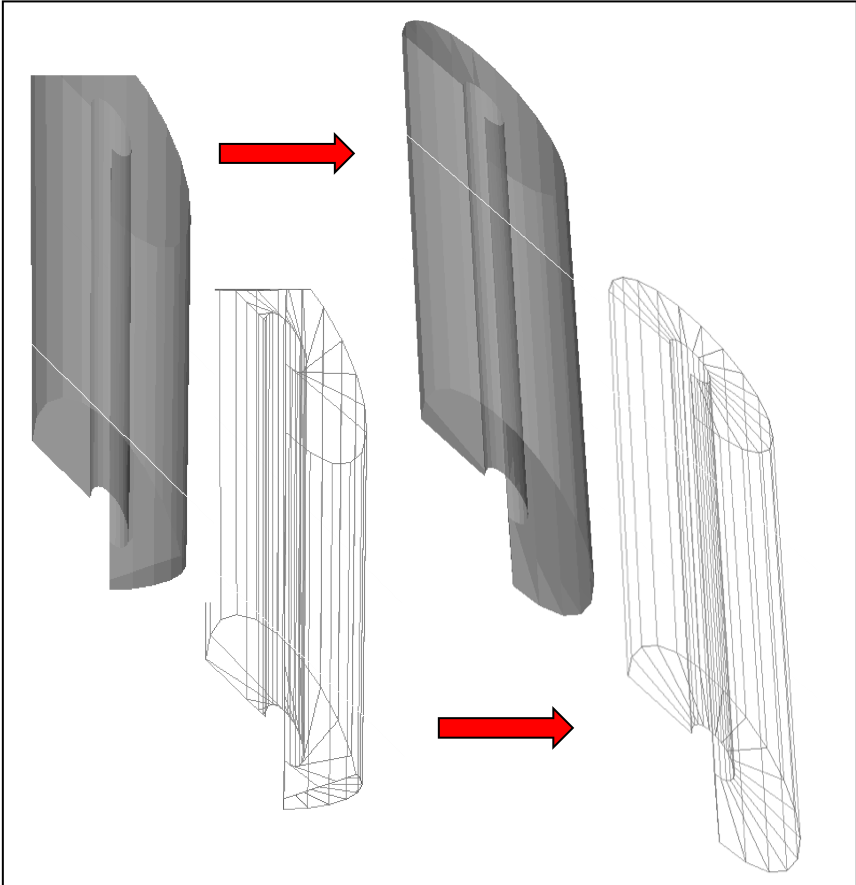
\includegraphics[height=1\linewidth]{Images//Meshes//CutTubs.png}
  \captionof{figure}{ }
  \label{ctub}
\end{minipage}%
\begin{minipage}{.3\textwidth}
  \centering
  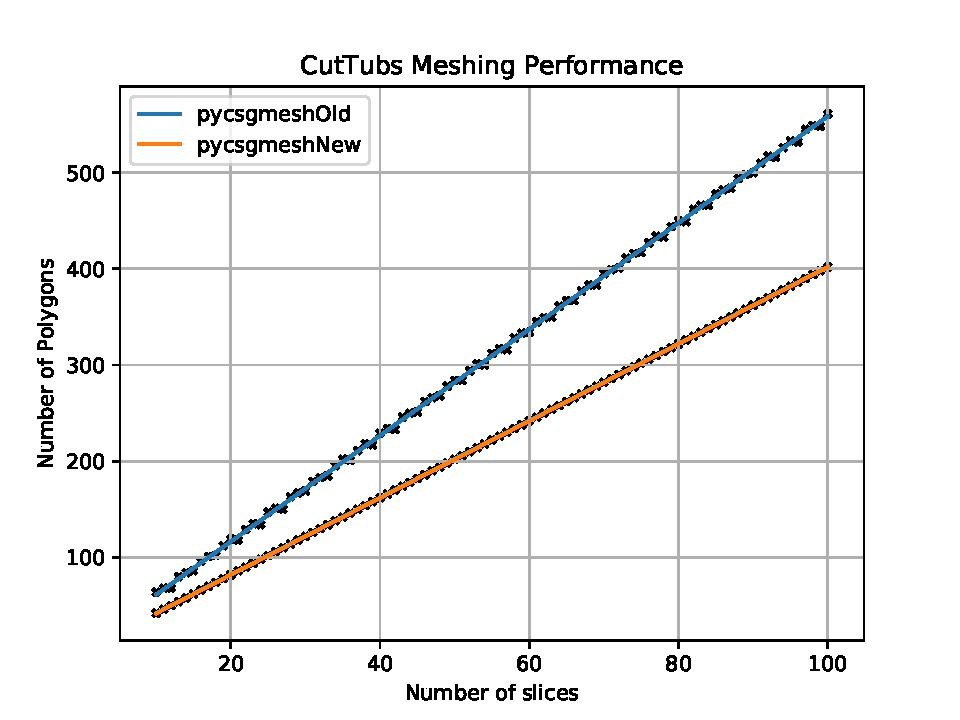
\includegraphics[scale=0.35]{Images//Quad_fits//CutTubs_quad.pdf}
  \captionof{figure}{ }
  \label{}
\end{minipage}%
\end{figure}

\subsubsection{Ellipsoid}

\begin{figure}[h!]
\centering
\begin{minipage}{.2\textwidth}
  \centering
  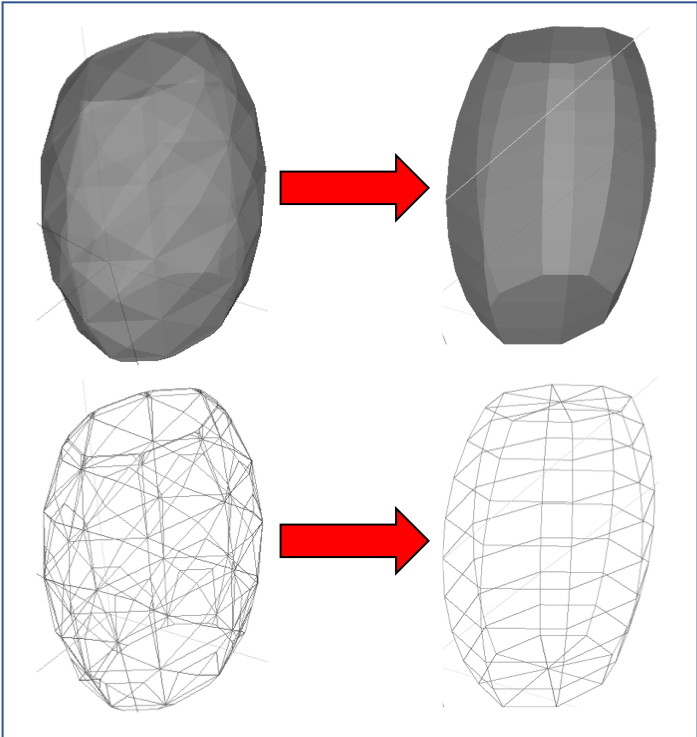
\includegraphics[height=1\linewidth]{Images//Meshes//ellipsoid.png}
  \captionof{figure}{ }
  \label{fig:test1}
\end{minipage}%
\begin{minipage}{.3\textwidth}
  \centering
  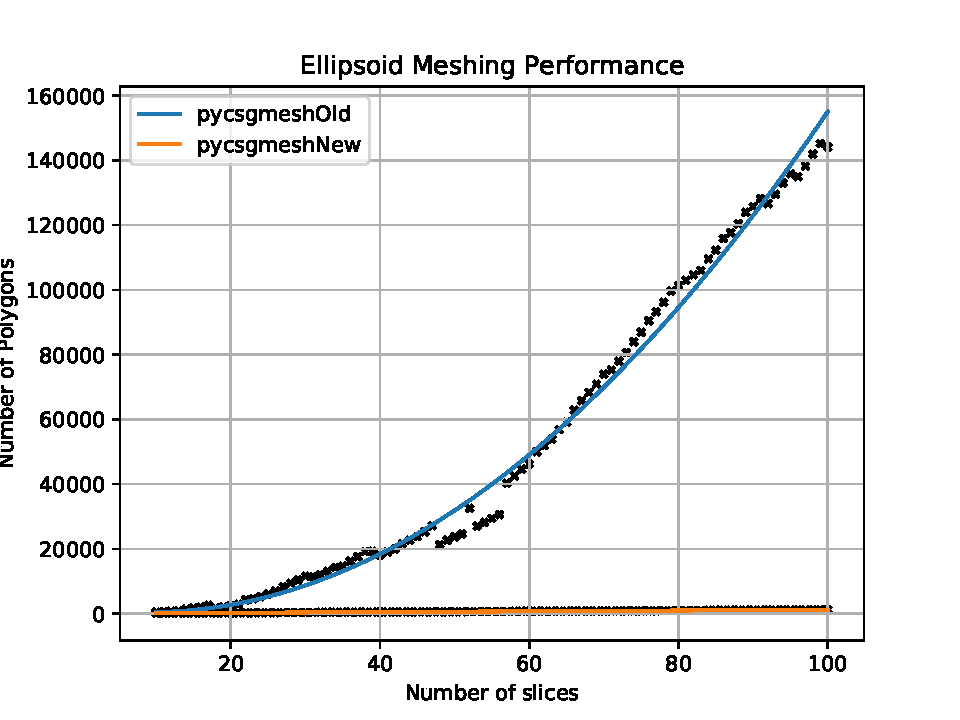
\includegraphics[scale=0.35]{Images//Quad_fits//Ellipsoid_quad.pdf}
  \captionof{figure}{ }
  \label{fig:test2}
\end{minipage}%
\end{figure}

\newpage
\subsubsection{EllipticalCone}

\begin{figure}[h!]
\centering
\begin{minipage}{.2\textwidth}
  \centering
  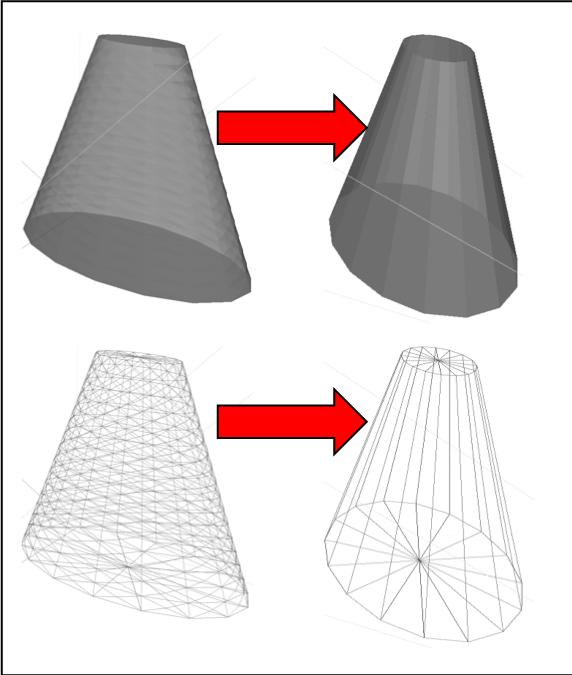
\includegraphics[height=1\linewidth]{Images//Meshes//ellipticalcone.png}
  \captionof{figure}{ }
  \label{fig:test1}
\end{minipage}%
\begin{minipage}{.3\textwidth}
  \centering
  \includegraphics[scale=0.35]{Images//Quad_fits//Ellipticalcone_quad.pdf}
  \captionof{figure}{ }
  \label{fig:test2}
\end{minipage}%
\end{figure}

\subsubsection{EllipticalTube}

\begin{figure}[h!]
\centering
\begin{minipage}{.2\textwidth}
  \centering
  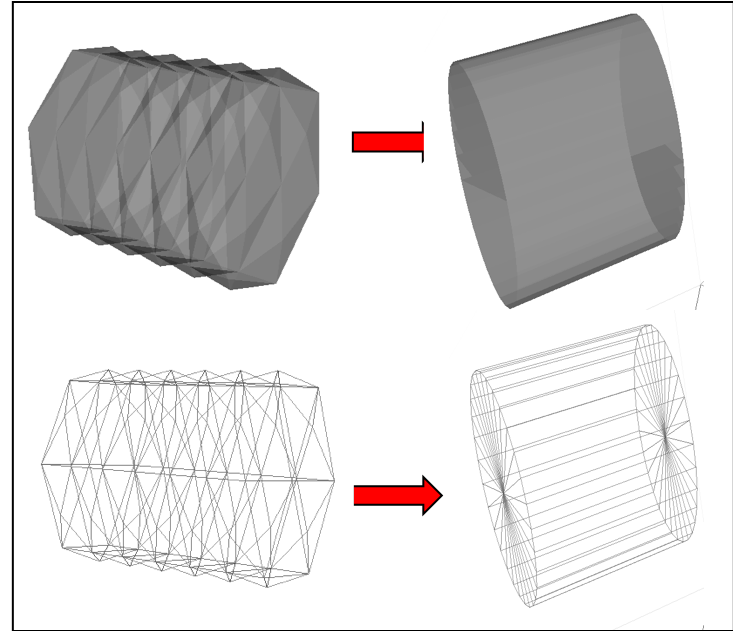
\includegraphics[height=0.8\linewidth]{Images//Meshes//ellipticaltube.png}
  \captionof{figure}{ }
  \label{fig:test1}
\end{minipage}%
\begin{minipage}{.3\textwidth}
  \centering
  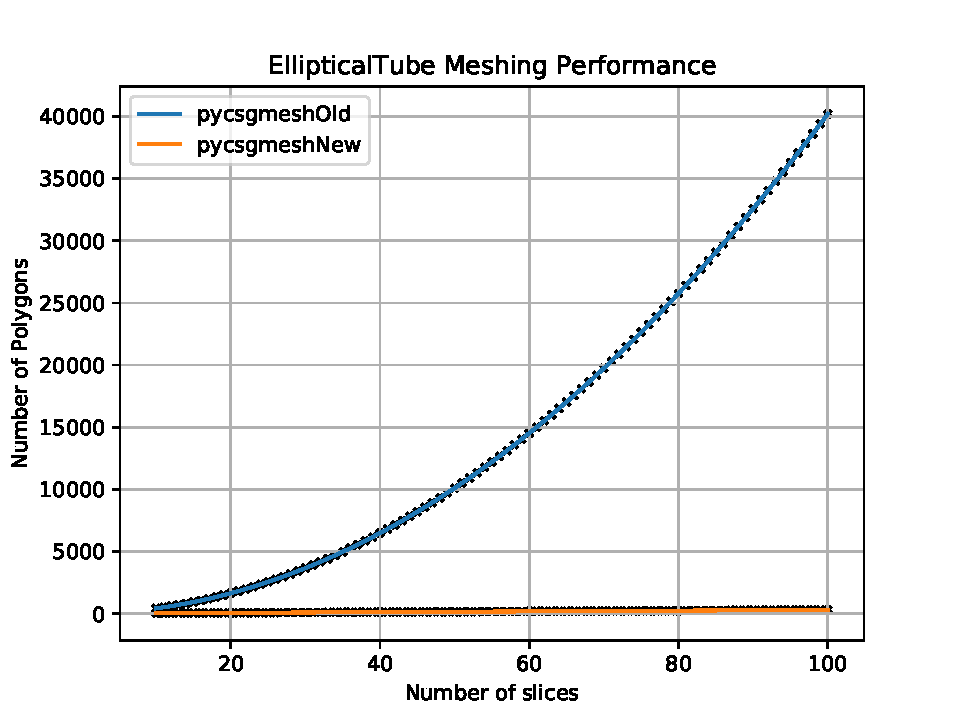
\includegraphics[scale=0.35]{Images//Quad_fits//EllipticalTube_quad.pdf}
  \captionof{figure}{ }
  \label{fig:test2}
\end{minipage}%
\end{figure}

\subsubsection{Hyperboloid}

\begin{figure}[h!]
\centering
\begin{minipage}{.2\textwidth}
  \centering
  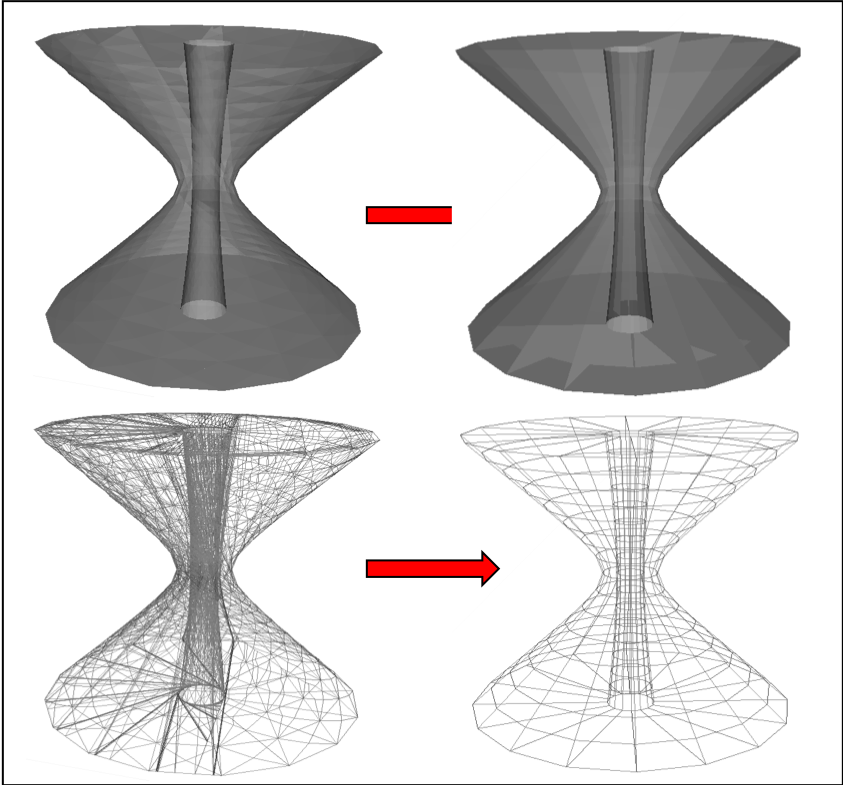
\includegraphics[height=0.9\linewidth]{Images//Meshes//hyperboloid.png}
  \captionof{figure}{ }
  \label{fig:test1}
\end{minipage}%
\begin{minipage}{.3\textwidth}
  \centering
  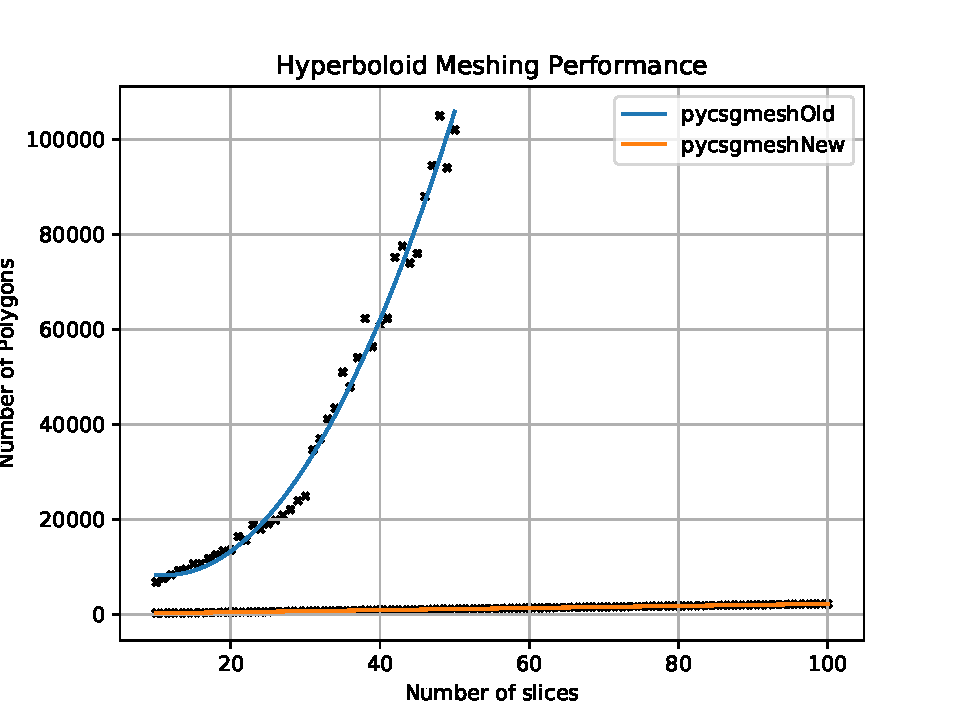
\includegraphics[scale=0.35]{Images//Quad_fits//Hyperboloid_quad.pdf}
  \captionof{figure}{ }
  \label{fig:test2}
\end{minipage}%
\end{figure}

\newpage
\subsubsection{Orb}

\begin{figure}[h!]
\centering
\begin{minipage}{.2\textwidth}
  \centering
  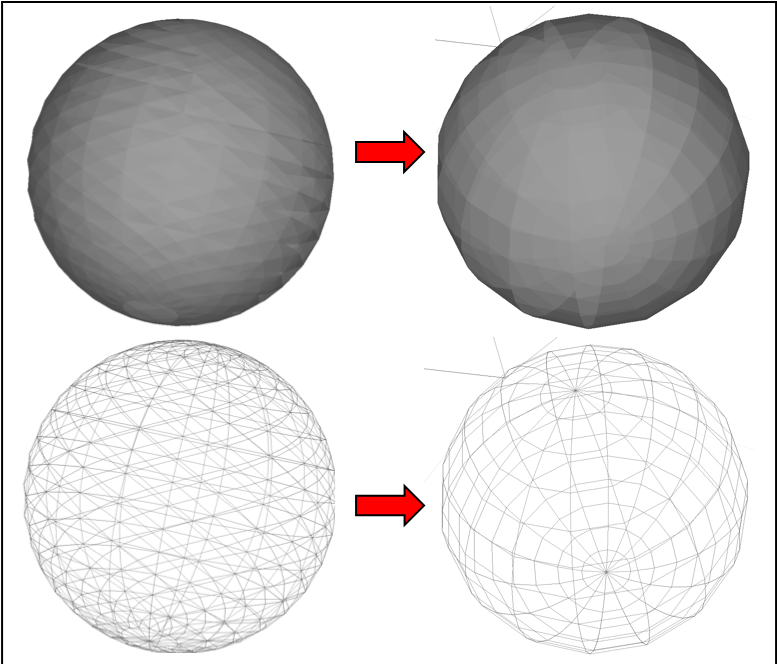
\includegraphics[height=0.8\linewidth]{Images//Meshes//orb.png}
  \captionof{figure}{ }
  \label{Sphere}
\end{minipage}%
\begin{minipage}{.3\textwidth}
  \centering
  \includegraphics[scale=0.35]{Images//Quad_fits//orb_quad.pdf}
  \captionof{figure}{ }
  \label{fig:test2}
\end{minipage}%
\end{figure}

\subsubsection{Paraboloid}

\begin{figure}[h!]
\centering
\begin{minipage}{.2\textwidth}
  \centering
  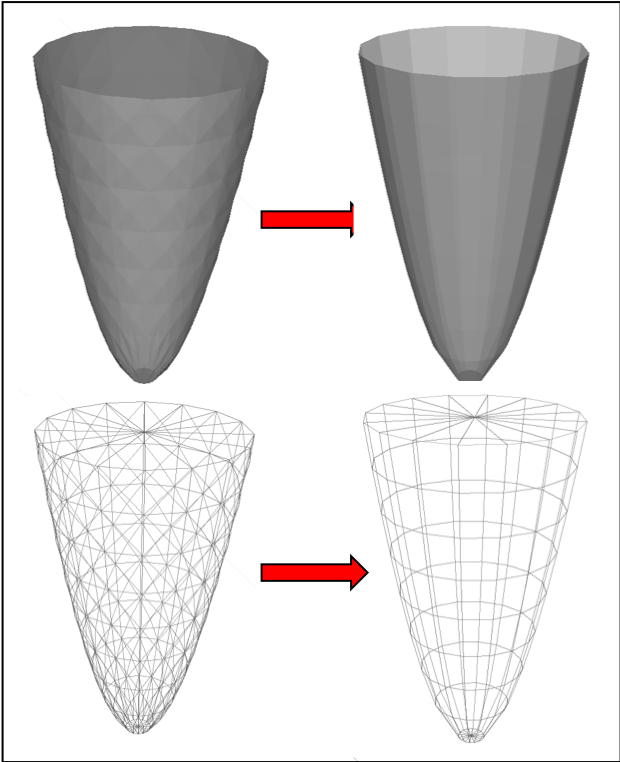
\includegraphics[height=1\linewidth]{Images//Meshes//paraboloid.png}
  \captionof{figure}{ }
  \label{para}
\end{minipage}%
\begin{minipage}{.3\textwidth}
  \centering
  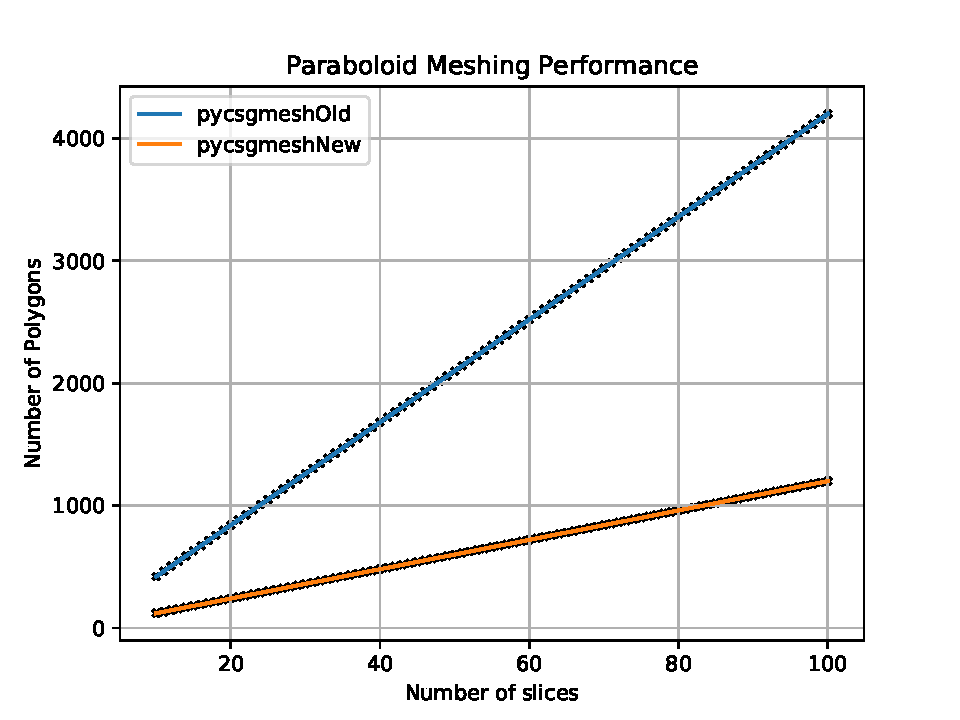
\includegraphics[scale=0.35]{Images//Quad_fits//Paraboloid_quad.pdf}
  \captionof{figure}{ }
  \label{fig:test2}
\end{minipage}%
\end{figure}

\subsubsection{Polycone}
\begin{figure}[h!]
\centering
\begin{minipage}{.2\textwidth}
  \centering
  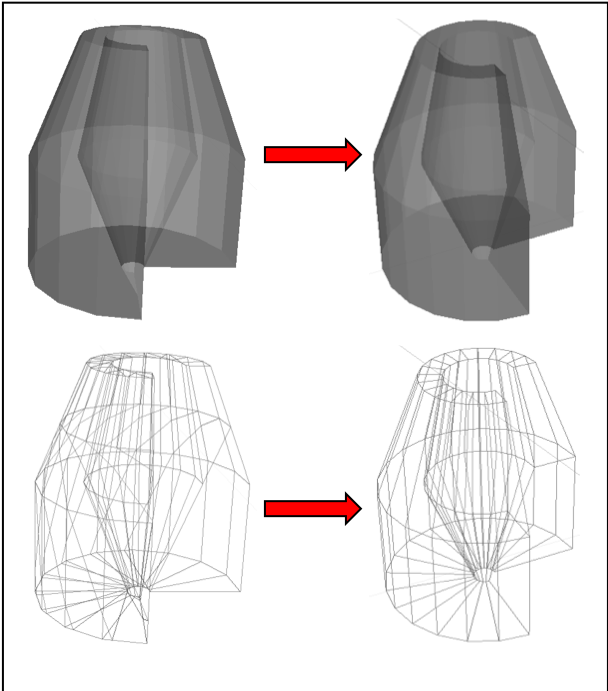
\includegraphics[height=1\linewidth]{Images//Meshes//polycone.png}
  \captionof{figure}{ }
  \label{fig:test1}
\end{minipage}%
\begin{minipage}{.3\textwidth}
  \centering
  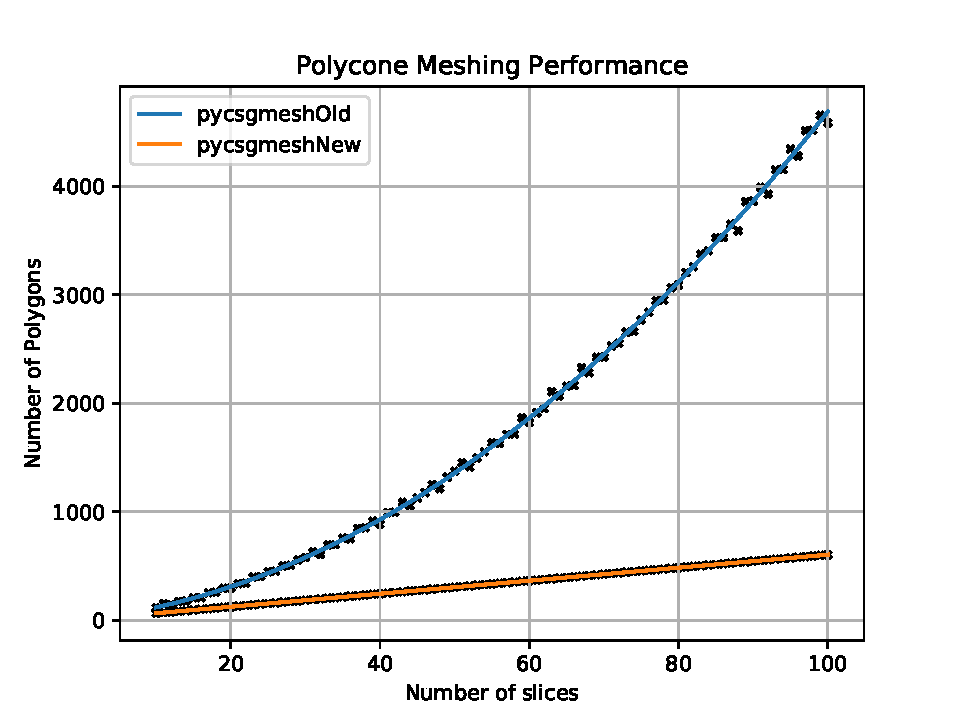
\includegraphics[scale=0.35]{Images//Quad_fits//Polycone_quad.pdf}
  \captionof{figure}{ }
  \label{fig:test2}
\end{minipage}%
\end{figure}

\newpage
\subsubsection{Sphere}
\begin{figure}[h!]
\centering
\begin{minipage}{.2\textwidth}
  \centering
  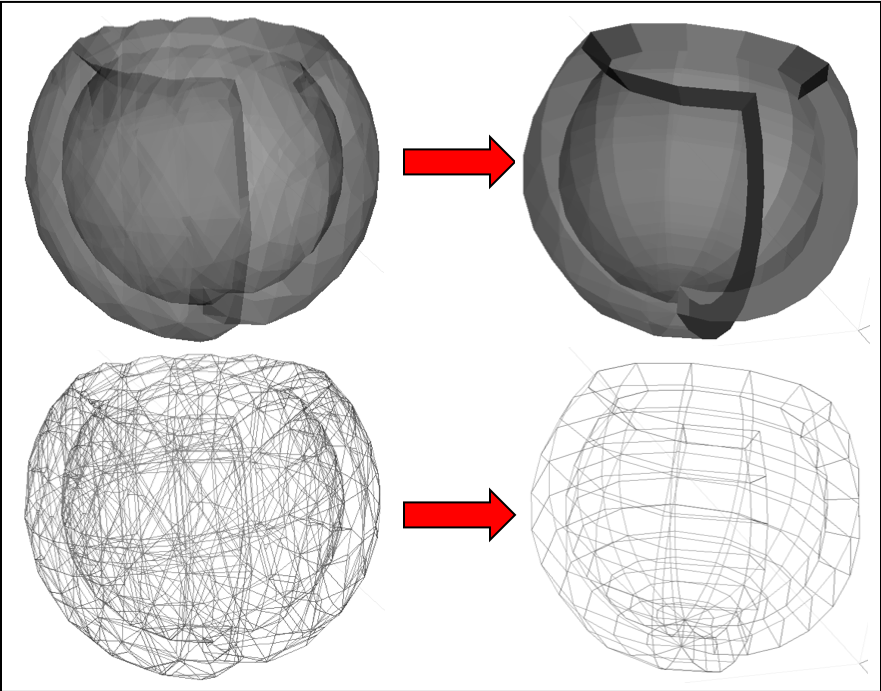
\includegraphics[height=0.75\linewidth]{Images//Meshes//sphere.png}
  \captionof{figure}{ }
  \label{fig:test1}
\end{minipage}%
\begin{minipage}{.3\textwidth}
  \centering
  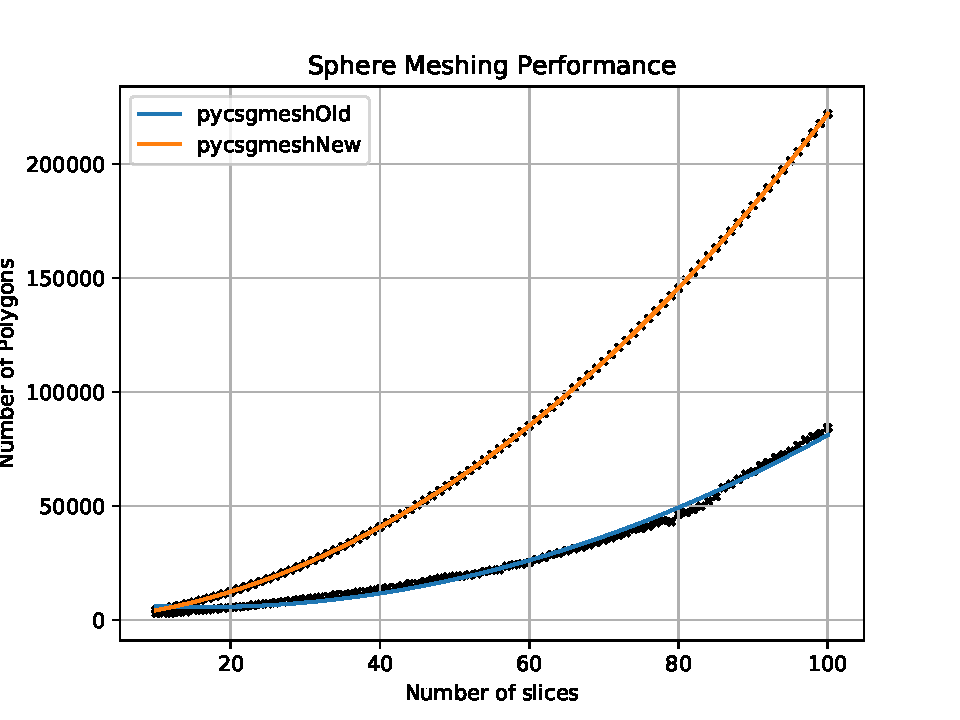
\includegraphics[scale=0.35]{Images//Quad_fits//Sphere_quad.pdf}
  \captionof{figure}{ }
  \label{fig:test2}
\end{minipage}%
\end{figure}

\subsubsection{Torus}

\begin{figure}[h!]
\centering
\begin{minipage}{.2\textwidth}
  \centering
  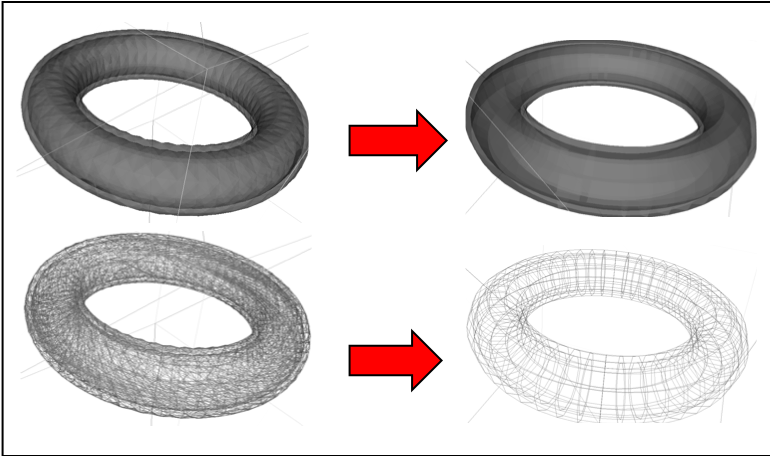
\includegraphics[height=0.5\linewidth]{Images//Meshes//torus.png}
  \captionof{figure}{ }
  \label{fig:test1}
\end{minipage}%
\begin{minipage}{.3\textwidth}
  \centering
  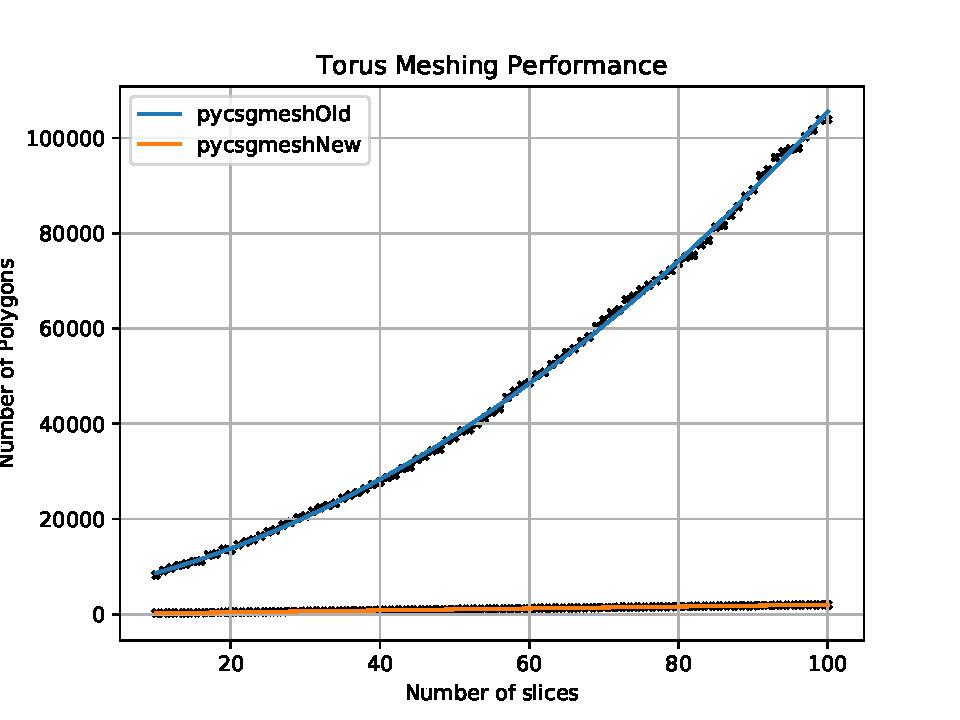
\includegraphics[scale=0.35]{Images//Quad_fits//Torus_quad.pdf}
  \captionof{figure}{ }
  \label{fig:test2}
\end{minipage}%
\end{figure}

\subsubsection{Tubs}

\begin{figure}[h!]
\centering
\begin{minipage}{.2\textwidth}
  \centering
  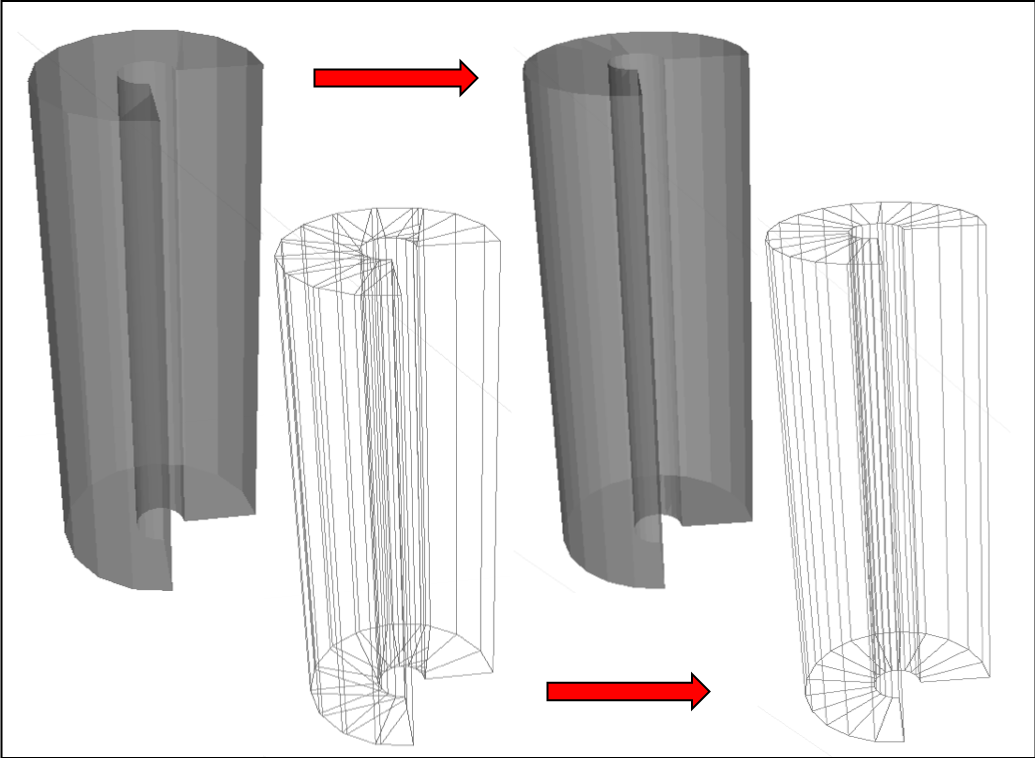
\includegraphics[height=0.7\linewidth]{Images//Meshes//tubs.png}
  \captionof{figure}{ }
  \label{fig:test1}
\end{minipage}%
\begin{minipage}{.3\textwidth}
  \centering
  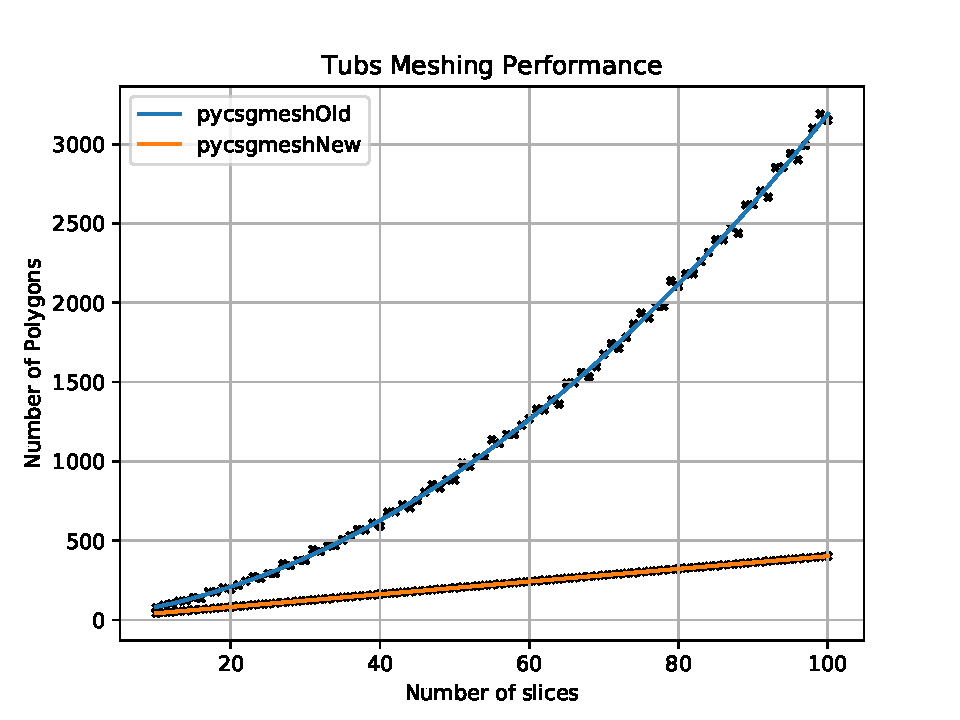
\includegraphics[scale=0.35]{Images//Quad_fits//Tubs_quad.pdf}
  \captionof{figure}{ }
  \label{fig:test2}
\end{minipage}%
\end{figure}

\endgroup
\onecolumn
\section{Quadratic Parameters for polygon count plots}
The quadratic fit where its parameters are of the form:
\begin{equation}
ax^2 + bx + c = 0
\end{equation}

\small
% Table generated by Excel2LaTeX from sheet 'Sheet1'
\begin{table}[htbp]
  \small
  \centering
  \caption{A Table showing the parameters to the quadratic fits for the polygon count plot.}
    \begin{tabular}{lrrrrrr}
    Curved Primitive Solid & \multicolumn{1}{l}{Old a} & \multicolumn{1}{l}{Old b} & \multicolumn{1}{l}{Old c} & \multicolumn{1}{l}{New a} & \multicolumn{1}{l}{New b} & \multicolumn{1}{l}{New c} \\
    Cons  & -2.74E-04 & 3.97E+00 & 5.72E+01 & -3.83E-17 & 4.00E+00 & 2.00E+00 \\
    CutTubs & 2.19E-04 & 5.50E+00 & 6.30E+00 & -3.83E-17 & 4.00E+00 & 2.00E+00 \\
    Ellipsoid & 18.65090372 & -333.5688153 & 1919.792901 & 1.61E-17 & 1.20E+01 & 0.00E+00 \\
    EllipticalCone & 4.00E+00 & 2.00E+00 & 2.41E-12 & 4.03E-18 & 3.00E+00 & 0.00E+00 \\
    EllipticalTube & -1.94E-16 & 4.20E+01 & -5.72E-13 & 4.03E-18 & 3.00E+00 & 0.00E+00 \\
    Hyperboloid & 64.83177713 & -1452.629624 & 16378.18198 & 4.84E-17 & 2.20E+01 & -9.53E-14 \\
    Orb   & -6.45E-17 & 3.40E+01 & -1.91E-13 & -8.06E-18 & 1.00E+01 & -4.77E-14 \\
    Paraboloid & -1.94E-16 & 3.40E+01 & -1.91E-13 & 1.61E-17 & 1.20E+01 & 0.00E+00 \\
    Polycone & 0.39682347 & 7.13011557 & 7.42466252 & -4.03E-17 & 6.00E+00 & 4.00E+00 \\
    Sphere & 10.82154926 & -356.6329124 & 8557.249195 & 2.00E+01 & 2.20E+02 & 1.98E-11 \\
    Torus & 7.01776508 & 304.8746037 & 4899.196225 & -1.61E-17 & 2.00E+01 & -9.53E-14 \\
    Tubs  & 0.27241769 & 4.58191175 & 8.33675211 & -3.83E-17 & 4.00E+00 & 2.00E+00 \\
    \end{tabular}%
  \label{tab1}%
\end{table}


\end{document}

